\documentclass[11pt]{scrartcl}

\title{Anforderungsspezifikation}
\author{Silvan Adrian \\ Fabian Binna \\ Pascal Kistler}
\date{\today{}}

\usepackage[ngerman]{babel}
\usepackage[automark]{scrpage2}
\usepackage{hyperref}
\usepackage{color}
\usepackage[normalem]{ulem}
\usepackage{scrpage2}
\usepackage{graphicx}
\usepackage{tabularx}
\usepackage{sidecap}
\graphicspath{ {./images/} }
\pagestyle{scrheadings}
\usepackage{wrapfig}
\usepackage{longtable, tabu}

\clearscrheadfoot
\ihead{
\includegraphics[scale=0.4]{jbomberman}}
\ohead{Projekt: JBomberman}
\ifoot{Anforderungsspezifikation}
\cfoot{Version: 1.09}
\ofoot{Datum: \today{}}
\setheadsepline{0.5pt}
\setfootsepline{0.5pt}

\usepackage{ucs}
\usepackage[utf8]{inputenc}
\usepackage[T1]{fontenc}


\begin{document}
\def\arraystretch{1.5}
\begin{titlepage}
\begin{center}
\vspace{10em}

\includegraphics[scale=2]{jbomberman}
\vspace{10em}
\end{center}
\begin{center}
\huge {Projekt: JBomberman} \\
\huge {Anforderungsspezifikation}
\end{center}
\begin{center}
\vspace{10em}
\LARGE {Pascal Kistler} \\
\LARGE {Silvan Adrian} \\
\LARGE {Fabian Binna}
\end{center}

\end{titlepage}

\newpage
\section{Änderungshistorie}
\label{sec:Änderungen}

\begin{tabularx}{\linewidth}{l l l l}
\textbf{Datum} & \textbf{Version} & \textbf{Änderung}  & \textbf{Autor} \\
\hline
\textbf{09.03.15} & 1.00 & Erstellung des Dokuments & Gruppe \\
\textbf{12.03.15} & 1.01 & detailliertes Spielprinzip geschrieben & Silvan Adrian \\
\textbf{13.03.15} & 1.02 & Spielregeln im Detail & Silvan Adrian \\
\textbf{17.03.15} & 1.03 & Allgemeine Beschreibung eingefügt & Silvan Adrian \\
\textbf{17.03.15} & 1.04 & Use Case beschrieben  & Pascal Kistler \\
\textbf{18.03.15} & 1.05 & Bilder ausgetauscht & Silvan Adrian \\
\textbf{19.03.15} & 1.06 & UseCase Diagram hinzugefügt & Pascal Kistler \\
\textbf{20.03.15} & 1.07 & Nichtfunktionale Anforderungen eingefügt & Silvan Adrian \\
\textbf{06.04.15} & 1.08 & Verbesserungen gemäss Reviewprotokoll & Silvan Adrian \\
\textbf{27.05.15} & 1.09 & Vorbereitung zur Abgabe & Silvan Adrian\\
\end{tabularx}

\newpage
\tableofcontents
\newpage
\section{Einführung}
\label{sec:Einführung}
\subsection{Zweck}
\label{sec:Zweck}
Dieses Dokument beschreibt die Anforderungen für das Projekt JBomberman.
\subsection{Gültigkeit}
\label{sec:Gültigkeit}
Dieses Dokument ist während des ganzen Projekts gültig und wird laufend aktualisiert.
\subsection{Referenzen}
\label{sec:Referenzen}
\begin{itemize}
  \item siehe letzte Seite Literatur
  \item Glossar
  \item Spielgrafiken : \href{http://gamedevelopment.tutsplus.com/articles/enjoy-
these-totally-free-bomberman-inspired-sprites--gamedev-8541}
{Tutsplus Gamedeveloopment}
\end{itemize}


\subsection{Übersicht}
\label{sec:Übersicht}
In diesem Dokument wird das Produkt hinsichtlich seiner Anforderungen 
beschrieben, dabei werden Einschränkungen, Annahmen, 
Abhängigkeiten und Funktionen beschrieben

\section{Allgemein Beschreibung}
\label{sec:Allgemeine Beschreibung}

\subsection{Produkt Perspektive}
\label{sec:Produkt Perspektive}
JBomberman soll ein kostenlos und einfach zu installierendes Spiel sein, 
das für alle Desktop Plattformen zur Verfügung steht.
Es soll für bis zu 4 Spieler kurzweilige Unterhaltung bieten.
\subsection{Produkt Funktion}
\label{sec:Produkt Funktion}
\begin{itemize}
    \item JBomberman ist ein Klon des Spielklassikers Bomberman
    \item JBomberman ist nur im Mehrspielermodus spielbar
    \item Es gibt einen dedizierten Server, der entweder lokal oder 
    auf einem entfernten Server gestartet werden kann
\end{itemize}

\subsection{Benutzer Chrakteristik}
\label{sec:Benutzer Chrakteristik}
Zur Zielgruppe von JBomberman gehören die, die  sich 
bereits für den Klassiker Bomberman interessiert haben.

In JBomberman wird vorausgesetzt das der Spieler schon einmal 
ein Netzwerkfähiges Spiel gespielt hat, da der Spieler selbst einen 
Server starten und sich über dessen IP oder FQDN verbinden muss.
\subsection{Einschränkungen}
\label{sec:Einschränkungen}
\begin{itemize}
    \item Es können maximal 4 Spieler an einem Spiel teilnehmen, 
    dabei geht das Spiel über mehrere Runden.
    \item Das Spiel soll auf allen gängigen Desktop Plattformen lauffähig sein.
    \item Ein Server kann nur 1 Spiel verwalten, somit benötigt
     jede Spielaustragung ihren eigenen Server
\end{itemize}
\subsection{Annahmen}
\label{sec:Annahmen}
\begin{itemize}
    \item Spielcomputer verfügt über Tastatur und Maus zur Steuerung
    \item Es wird vorausgesetzt, dass der Spieler mit den Spielregeln vertraut ist
\end{itemize}

\subsection{Abhängigkeit}
\label{sec:Abhängigkeit}
Die lauffähigkeit von JBomberman hat direkte einbussen, wenn 
folgende Abhängigkeiten nicht erfüllt sind.
\begin{itemize}
    \item Es wird Java in der Version 8 vorausgesetzt
    \item Der Spielcomputer muss sich entweder im gleichen Netzwerk 
    wie der Server befinden oder Zugriff aufs Internet haben
    \item Die Performance hängt von der zur Verfügung stehenden 
    Bandbreite zum Server und der Geschwindigkeit von RabbitMQ 
    beim abarbeiten der Queues ab
\end{itemize}

\newpage
\section{Detailiertes Spielprinzip}
\label{sec:Detailiertes Spielprinzip}
\subsection{Kurzbeschreibung}
\label{Kurzbeschreibung}
In der klassischen Variante besteht das Spielfeld aus einer Anordnung 
von zerstörbaren und unzerstörbaren Wänden. 
Durch das Legen von Bomben können somit immer mehr 
Bereiche des Spielfelds erschlossen werden. Hinter einigen 
Wänden verstecken sich Bonusgegenstände.\cite{Bomberman Spielprinzip}

\subsection{Spielregeln}
\label{sec:Spielregeln}

\subsubsection{Spielewinn}
\label{sec:Spielgewinn}
Ein Spieler hat gewonnen, wenn alle anderen Bombermans besiegt sind und er der 
letzte bestehende Spieler auf dem Spielfeld ist.
Der Gewinner bekommt einen Punkt für die gewonnene Runde (round) 
und wird im angerechnet angezeigt in der Statusanzeige.
Der Bomberman mit den meisten gewonnen Runden hat ist schlussendlich der Gewinner.
Die Anzahl maximal Runden ist festgelegt durch maxRounds.

\subsubsection{Spielabbruch}
\label{sec:Spielabbruch}
Zu einem Spielabbruch kommt es, wenn es zu wenige Mitspieler gibt 
(mindestens 2 Spieler müssen verbunden sein und Ready).

\subsubsection{Timer läuft ab}
\label{sec:Timer läuft ab}
Falls innerhalb der festgelegten Zeit kein Bomberman alle anderen Mitspieler besiegt 
kriegen die Bombermans die vollen PowerUps.
Der Bomberman, der übrig bleibt wird dabei der Gewinner der Spielrunde.

\subsubsection{Bombe}
\label{sec:Bombe}
Sobald eine Bombe platziert ist wird dessen \grqq{}Zeit 
bis zur Explosion gestartet\grqq{}.
Sobald ein Bombe explodiert wird alles was sich im Radius 
(bombPower) der Bombe befindet und zerstörbar ist zerstört.
Der Radius der Bombenexplosion kann varieren, da Powerups 
für das Erhöhen des Bombenradius bestehen.
\subsubsection{Zerstörbare Wand}
\label{sec:Zerstörbare Wand (DestroyableBlock)}
Wenn eine zerstörbare Wand zerstört wird verschwindet diese und macht den Weg frei.
Manche zerstörbaren Wände verbergen Powerups für die Bombermans, 
welche nach dem zerstören der Wand aufgedeckt werden.
Solange die Wand aber nicht zerstört ist kann auch kein Bomberman diese durchqueren.

\subsubsection{Unzerstörbare Wand}
\label{sec:Unzerstörbare Wand}
Unzerstörbare Wände können nicht durch Bomben zerstört werden, 
noch von Bombermans durchquert werden.

\subsubsection{Bomberman}
\label{sec:Bomberman}
Der Bomberman wird über die Tastatur gesteuert, dabei gibt es 4 
Tasten für die Fortbewegung und 1 Zusätzliche Taste für das legen der Bombe.
Ein Bomberman kann sich \grqq{}upgraden\grqq{}, wenn er Powerups aufhebt.

\subsection{Spielelemente}
\label{sec:Spielelemente}
Jedes Spielelement hat visuelle Element, welche als Sprites bezeichnet werden.
Zusätzlich hat jedes Spielelement eine Position, wo dieses platziert wird, 
wie auch einen festgelegten Namen.
Dabei gibt es auch animierte Elemente (AnimatedSprites), wie Explosionen, 
Bomben oder die Bombermans selbst, die wiederum verschiedene Geschwindigkeiten 
(animationSpeed) haben können.
\subsubsection{Statusanzeige}
\label{sec:Statusanzeige}
In der Statusanzeige wird für jeden einzelnen Bomberman (2-4 Spieler) die Anzahl 
Gewinne, ein Timer der runterzählt und die momentane Runde angezeigt.
\subsubsection{Spielfeld}
\label{sec:Spielfeld}
Das Spielfeld wird sich auf eine Grösse von ca. 13 Blöcken x 13 Blöcken 
erstrecken.
Die Wände sind dabei unzerstörbar, damit die bis zu 4 Bombermans das Spielfeld 
nicht verlassen können.
Jeder Ecken im Spielfeld ist für einen Bomberman festgelegt, bei weniger als 4 
Spielern bleiben die übrigen Ecken leer.
\begin{center}
Spielfeld in JBomberman mit 4 Spielern.
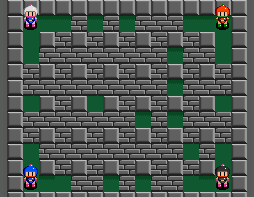
\includegraphics[scale=1.4]{bombermanmap} 
\end{center}

\newpage
\subsection{Wände}
\label{sec:Wände}
\subsubsection{Unzerstörbar}
\label{sec:Unzerstörbar}
\begin{table}[!h]
\begin{tabularx}{\linewidth}{l X }
     
      \raisebox{-.8\totalheight}{ 
\includegraphics[scale=.8]{solidblock}}
      & Die unzerstörbaren Wände können von keiner Bombe zerstört noch von einem 
Bomberman durchlaufen werden.
\end{tabularx}
\end{table}


\subsubsection{Zerstörbar}
\label{sec:Zerstörbar}

\begin{table}[!h]
  \begin{tabularx}{\textwidth}{l X }
    
    
       \raisebox{-.8\totalheight}{
\includegraphics[scale=0.8]{explodableblock}} & 
       Die zerstörbaren Wände können von 
    einer Bombe zerstört werden, bevor sie zerstört sind kann ein Bomberman 
    diese nicht durchlaufen.
  \end{tabularx}
\end{table}
\subsection{Bomberman (Player)}
\label{sec:Bomberman}
\begin{table}[!h]
\begin{tabularx}{\textwidth}{l X}
\raisebox{-.8\totalheight}{
\includegraphics[scale=0.6]{bomberman}}
  & Der Bomberman ist der steuerbare Charakter im Bomberman Spiel, dabei kann er 
sich in alle Himmelsrichtungen bewegen.
Es sei denn ein Hindernis ist im Weg, dann kann er sich nicht weiter bewegen.
Jeder Bomberman hat einen eindeutigen Namen (name) und eine 
Anzahl gewonnen Runden (score).
\end{tabularx}
  
\end{table}



\subsection{Bombe}
\label{sec:Bombe}
\begin{table}[!h]
\begin{tabularx}{\textwidth}{l X}
\raisebox{-.8\totalheight}{
\includegraphics[scale=0.8]{bomb}}
& Die Bombe ist wohl der wichtigste Gegenstand im JBomberman, denn ohne die Bombe 
könnten sich die Bombermans ihren Weg nicht freiräumen.
Somit ist die Funktion der Bombe das beseitigen von zerstörbaren Wände und um 
Gegenspieler frühzeitig aus dem Spiel zu werfen.
\end{tabularx}

\end{table}
\newpage
\subsection{Power Ups}
\label{subsec:Power Ups}
Durch zerstören, der zerstörbaren Wände kommen Power Ups zutage, welche einen 
gewissen Einfluss auf das Spielerlebnis haben.

\subsubsection{Bombe}
\label{sec:Bombe}
\begin{table}[!h]
\begin{tabularx}{\textwidth}{l X}
\raisebox{-.6\totalheight}{
\includegraphics[scale=0.8]{bombpowerup}}
& Durch dieses Powerup ist es dem Bomberman möglich mehr als eine 
Bombe zu platzieren, dabei gibt es ein Maximum von Bomben 
(maxBombs) welche zur gleichen Zeit gelegt werden können.
\end{tabularx}
\end{table}

\subsubsection{Stiefel}
\label{sec:Stiefel}
\begin{table}[!h]
\begin{tabularx}{\textwidth}{l X}
\raisebox{-.6\totalheight}{
\includegraphics[scale=0.8]{speedpowerup}}
& Durch dieses Powerup beschleunigt sich die Fortbewegungsgeschwindigkeit 
(movementSpeed) eines Bomberman.
\end{tabularx}

\end{table}

\subsubsection{Flamme}
\label{sec:Flamme}

\begin{table}[!h]
\begin{tabularx}{\textwidth}{l X}
\raisebox{-.6\totalheight}{
\includegraphics[scale=0.8]{flamepowerup}}
& Dieses Powerup gibt der Bombe einen grösseren Sprengradius (bombPower) 
-> (in alle 4 Himmelsrichtungen) -> (Explosion).

\end{tabularx}

\end{table}

\newpage
\section{Use Cases}
\label{sec:Use Cases}

\subsection{Use Case Diagramm}
\label{sec:Use Case Diagramm}
\raisebox{-.6\totalheight}{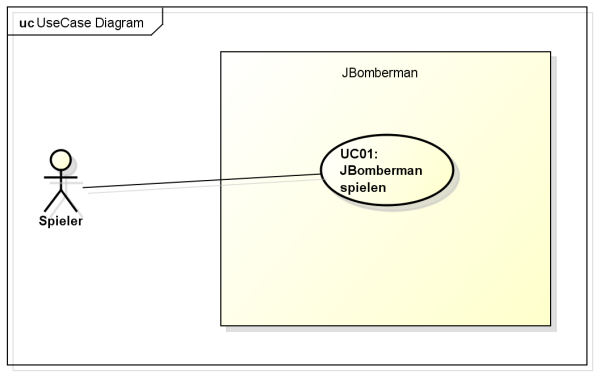
\includegraphics[scale=0.8]{UCDiagram}}

\subsection{Aktoren + Stakeholders}
\label{Aktoren + Stakeholders}
  	\begin{tabularx}{\linewidth}{lll}
  		\bfseries Aktor & \bfseries Typ & \bfseries Ziele \\\hline 
  		Spieler & Primary &  
  		\begin{minipage}{5in}
  			\vskip 4pt
  			\begin{itemize}
  				\item Einfach mit Server verbinden
  				\item Ohne Umwege Spiel starten
  				\item Schnelle Beendigung des Spiels
  				\item Schnelle Reaktionszeit des Spiels
  				\item kurzweilige Unterhaltung
  			\end{itemize}
  			\vskip 4pt
  		\end{minipage}
		\\ \hline
	\end{tabularx}

\newpage
\subsection{Beschreibungen fully dressed}
\label{sec:Beschreibungen full dressd}

\subsubsection{UC01: JBomberman spielen}
\label{sec:UC01: JBomberman spielen}
\belowtabulinesep = 1mm
\begin{longtabu} to \textwidth {X[1,l] X[2,l]}
	\bfseries Primäraktor & Spieler  \\\hline 
	\bfseries Steakholders und Interessen & Spieler: Möchte das Spiel gemeinsam mit Bekannten spielen  \\\hline 
	\bfseries Vorbedingungen & Das Programm wurde gestartet  \\\hline 
	\bfseries Nachbedingungen & Das Programm wurde beendet  \\\hline 
	\bfseries Standartablauf & 
		\begin{enumerate}
			\item Der Spieler gibt die Adresse des Servers ein zu dem er sich verbinden möchte
			\item Spieler drückt auf \textbf{Connect}
			\item Die Verbindung wird hergestellt und andere evtl. wartende Spieler werden in der Lobby angezeigt
			\item Der Spieler klickt \textbf{I'm ready}
			\item Sobald alle Spieler bereit sind, wird das Spiel gestartet
			\item Die Spielumgebung wird gestartet und die erste Runde beginnt
			\item Bis zur letzten Runde wiederholen
			\begin{enumerate}
				\item Der Countdown zu Beginn einer Runde gibt den Spielern Zeit sich und die andern Spieler zu lokalisieren. Nach dem Countdown kontrollieren die Spieler ihre Figur und die Runde beginnt
				\item Am Ende einer Runde wird jedem Spieler angezeigt, ob er gewonnen hat und der Punktestand aller Spieler
			\end{enumerate}
			\item Die Spielumgebung wird beendet und der Spieler befindet sich wieder in der Lobby
			\item Der Spieler verlässt die Lobby indem er auf \textbf{Disconnect} drückt
			\item Der Spieler schliesst das Verbindungsfenster
		\end{enumerate}
\\\hline 
	\bfseries Alternativer Ablauf & 
		\begin{enumerate}
			\setcounter{enumi}{1}
			\item 
			\begin{enumerate}
				\item Der Server ist nicht erreichbar. Das System gibt eine Fehlermeldung aus und der Spieler kann eine andere Adresse angeben (Schritt 1)
			\end{enumerate}
			\item 
			\begin{enumerate}
				\item Der Spieler entscheidet sich um
				\begin{enumerate}
					\item Der Spieler drückt auf \textbf{Disconnect}. 
					\item Die Verbindung wird getrennt und der Spieler befindet sich wieder auf dem Startbildschirm (Schritt 1)
				\end{enumerate}
			\end{enumerate}
			\item 
			\begin{enumerate}
				\item Der Spieler entscheidet sich um
				\begin{enumerate}
					\item Der Spieler drückt auf \textbf{I'm not ready}. 
					\item Solange mindestens ein Spieler nicht bereit ist, startet das Spiel nicht. (Schritt 3)
				\end{enumerate}
			\end{enumerate}
			\setcounter{enumi}{6}
			\item 
			\begin{enumerate}
				\item 
				\begin{enumerate}
					\item Der Spieler schliesst das Fenster
					\item Das Spiel beendet sich und der Startbildschirm erscheint (Schritt 1)
				\end{enumerate}
			\end{enumerate}
		\end{enumerate}  \\\hline 
	\bfseries Spezielle Anforderungen & siehe nichtfunktionale Anforderungen  \\\hline 
	\bfseries Technologie- und Datenvarianten & Keine  \\\hline 
	\bfseries Auftrittshäufigkeit & mehrmals pro Woche  \\\hline 
	\bfseries Offene Fragen & Keine  \\\hline  
\end{longtabu}

\newpage
\section{Nichtfunktionale Anforderungen}
\label{sec:Nicht funktionale Anforderungen}


\subsection{Menge}
\label{sec:Menge}
\begin{itemize}
    \item Anzahl Spieler ist beschränkt (auf 4)
    \item Bombenanzahl ist beschränkt (auf 8 pro Bomberman)
    \item Anzahl Runden werden festgelegt (3 Runden)
    \item Spielzeit wird festgelegt (3 min)
\end{itemize}



\subsubsection{Schnittstellen}
\label{sec:Schnittstellen}
\begin{itemize}
    \item Zur Interaktion mit dem Spieler werden herkömmliche Schnittstellen benötigt 
    (Maus, Tastatur, Bildschirm)
    \item Das System benötigt eine Netzwerkschnittstelle, um mit den 
    anderen Spielern Kommunizieren zu können.
    \item Es wird ein gestartet Server gebraucht, welcher über seine IP oder FQDN
     erreichbar ist
\end{itemize}

\subsection{Qualitätsmerkmale}
\label{sec:Qualitätsmermale}

\subsubsection{Funktionalität}
\label{sec:Funktionalität}
siehe Detailiertes Spielprinzip


\subsubsection{Zuverlässigkit}
\label{sec:Zuverlässigkeit}
\begin{itemize}
    \item JBomberman bietet nur einen Mehrpsielermodus und
     dieser soll in 90\% der Fälle durchführbar sein.
    \item Falls ein Spieler die Netzwerkverbindung verliert, wird 
    dieser aus dem laufenden Spiel geworfen.
    \item Die restlichen Spieler können dabei weiterspielen.
\end{itemize}

\subsubsection{Benutzbarkeit}
\label{sec:Benutzbarkeit}
\begin{itemize}
    \item JBomberman verfügt über ein User Interface, was ein 
    einfaches einsteigen ins Spiel ermöglichen soll
    \item Das Spiel selbst wird nur mit der Tastatur gesteuert
\end{itemize}

\subsubsection{Effizienz}
\label{sec:Effizienz}
\begin{itemize}
    \item Server muss sich 30 mal in der Sekunde updaten und
     im gleichen Intervall Messages versenden können
    \item Client muss im gleichen Interval alles rendern können
\end{itemize}

\subsubsection{Änderbarkeit}
\label{sec:Änderbarkeit}
Für JBomberman sind vorerst keine Erweiterungen geplant, 
weitere PowerUps wären allerdings denkbar.


\subsubsection{Übertragbarkeit}
\label{sec:Übertragbarkeit}
Da das Projekt in Java umgesetzt wird ist es Plattformunabhängig, 
dadurch kann es auch von verschiedenen Spielern auf anderen 
Plattformen gespielt werden.
In unserem Team selbst sind auch 3 verschiedene Entwicklungsumgebungen 
vorhanden, wodurch es noch wichtiger ist das die Plattformunabhängigkeit gegeben ist.



\begin{thebibliography}{999}
\bibitem [Spielprinzip] {Bomberman Spielprinzip}
\url{http://de.wikipedia.org/wiki/Bomberman}, Zugriff 
11.03.2015
\end{thebibliography}

\end{document}